\documentclass[
a4paper, 
12pt, 
]{article}

% \usepackage[ngerman,english]{babel}			% Kapitel/Chapter. typographic rules
\usepackage[english]{babel}



\usepackage[utf8]{inputenc}			% Encoding with umlauts and ß
%\usepackage{lipsum}				 			% testing text as \lipsum[1-3] 			 
%\usepackage{titling}							% imports \theauthor
\usepackage{graphicx}						% include graphics
\usepackage{siunitx}							% corretct formatting of units
\usepackage[framed,numbered,autolinebreaks,useliterate]{mcode} % for matlab code

\usepackage{amsmath}            % nice equations
\usepackage{url}                			% URLs
%\usepackage{natbib}             		% author-year bibliography style
\usepackage{hyperref}           	% PDF links
%\usepackage{subfig}             	% Subfigures (a), (b), etc
%\usepackage{nomencl}            	% Nomenclature	
\usepackage{tcolorbox}
\usepackage{Systemtheorie}		 	% style with headers/footers/logo/firstpage
\fancyfoot[R]{Juri Fedjaev} 
\usepackage{units}		% nice fractions using \nicefrac
\usepackage{blindtext}
\usepackage{mcode}
\usepackage[update,prepend]{epstopdf}
% ----------------------------------------------------------------------------


\begin{document}
	
	\thispagestyle{firstpage} 			% use different style here (from .sty file)
	
	\section*{Neuroprothetik -- Exercise 3: Mathematical Basics II}
	\subsection{Implementations in Matlab or Python}
	\subsubsection{Forward (Explicit) Euler}
	The forward Euler has been implemented as a function in Matlab (\mcode{function [V, t] = forwardEuler(h, N, DGL, V_0, t_0)}). The input variables are the step length \mcode{h}, the maximum time length \mcode{N}, a function handle to a differential equation \mcode{DGL}, starting value for the voltage \mcode{V_\0} and the starting point for the time vector \mcode{t_\0}. \emph{See code for more detailed information.} 	
	\subsubsection{Heun Method}
	The Heun method has been implemented as a function in Matlab (\mcode{function [V, t] = heunMethod(h, N, DGL, V_0, t_0)}). The input variables have been described previously.
	\emph{See code for more detailed information.} 
	\subsubsection{Exponential Euler}
	The exponential Euler has been implemented as a function in Matlab (\mcode{function [V, t] = exponentialEuler(h, N, A, B, V_0, t_0)}). The input variables are basically the same as stated before, except for the function handle \mcode{DGL}, which is now divided into to function handles \mcode{A} and \mcode{B}, as presented in the lecture. \emph{See code for more detailed information.} 
	
	\subsection{Solve Functions}
	In this section the differential equation from the previous problem sheet will be solved: 
	\begin{align}
	\frac{dV}{dt} &= 1 - V - t.
	\end{align}
	The starting point is $V(t_0) = V(-4.5) = V_0 = -4$. The step size will be $h \in \{1s, 0.5s, 0.1s, 0.012s\}$. 
	
	\subsubsection{Forward (Explicit) Euler}
	The results for the \emph{forward Euler} are shown in fig.~\ref{fig:ForwardEuler}. The larger the step size, the bigger is the overshoot at the local maximum for that function. Smaller step sizes yield better results, i.e. approximate the curve much better. For $h = 1s$ there is an undershoot, but still the curve looks better

\begin{figure}[h]
\centering
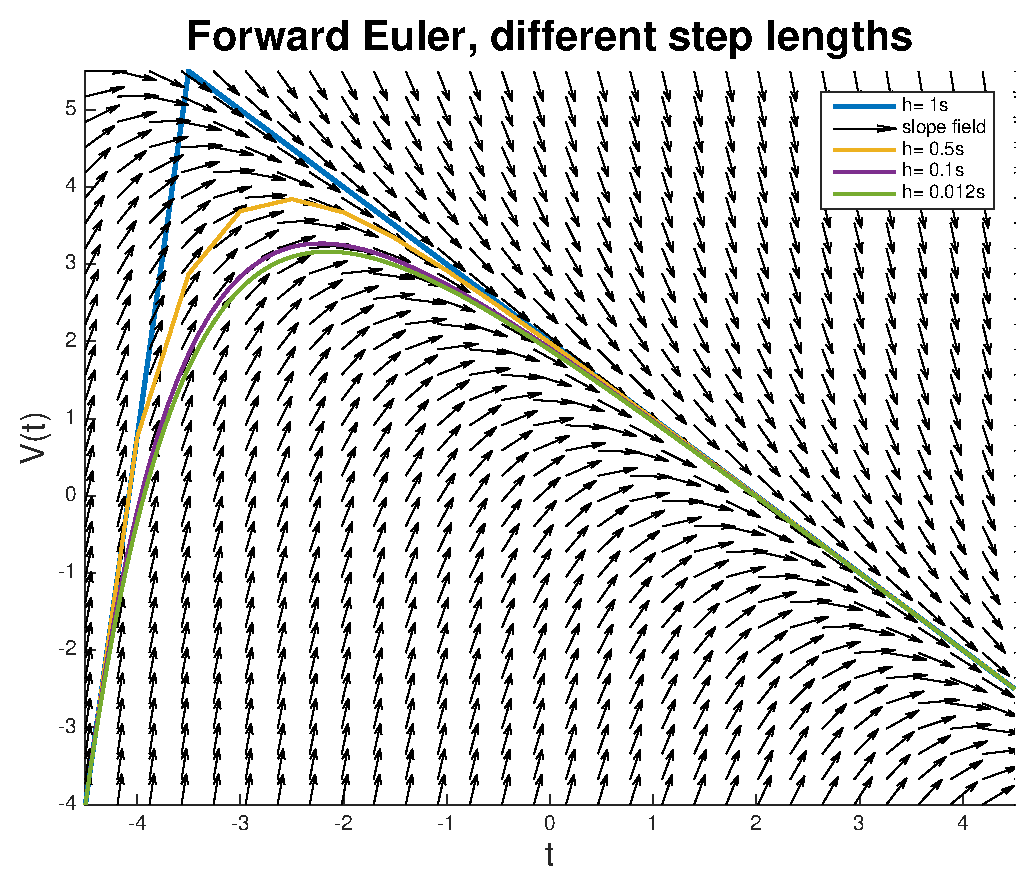
\includegraphics[width=0.85\linewidth]{Plots/ForwardEuler}
\caption{Forward Euler with different step sizes.}
\label{fig:ForwardEuler}
\end{figure}



\clearpage
	\subsubsection{Heun Method}
	The results for the \emph{Heun method} are shown in fig.~\ref{fig:HeunMethod}. When compared to the forward Euler, the Heun method converges faster. The curves for $h = 0.012s$ and $h = 0.1s$ even overlap completely in the figure. Here, the low step size $h = 1s$ yields an undershoot, but looks smoother overall. 
	
	\begin{figure}[h]
		\centering
		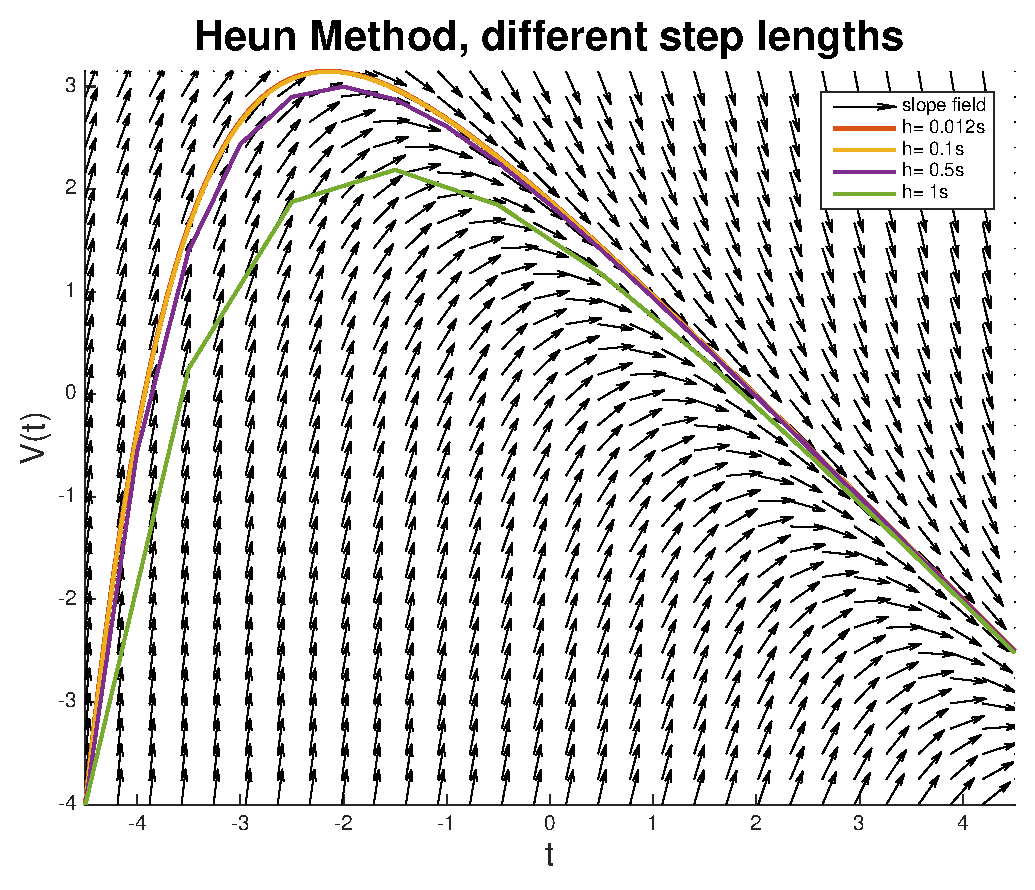
\includegraphics[width=0.85\linewidth]{Plots/HeunMethod}
		\caption{Heun method with different step sizes. The plots for $h = 0.012s$ and $h = 0.1s$ are overlapping and thus not well distinguishable. }
		\label{fig:HeunMethod}
	\end{figure}
	
		
	
	\clearpage
	\subsubsection{Exponential Euler}
	The results for the \emph{Exponential Euler} are shown in fig.~\ref{fig:ExpEuler}. The exponential Euler exhibits a constant offset with large step sizes (e.g. \mcode{h = 1}s). This offset gets smaller with increasingly small step sizes. However, the approximation looks the best overall when neglecting the offset for the bigger step sizes. 

	\begin{figure}[h]
		\centering
		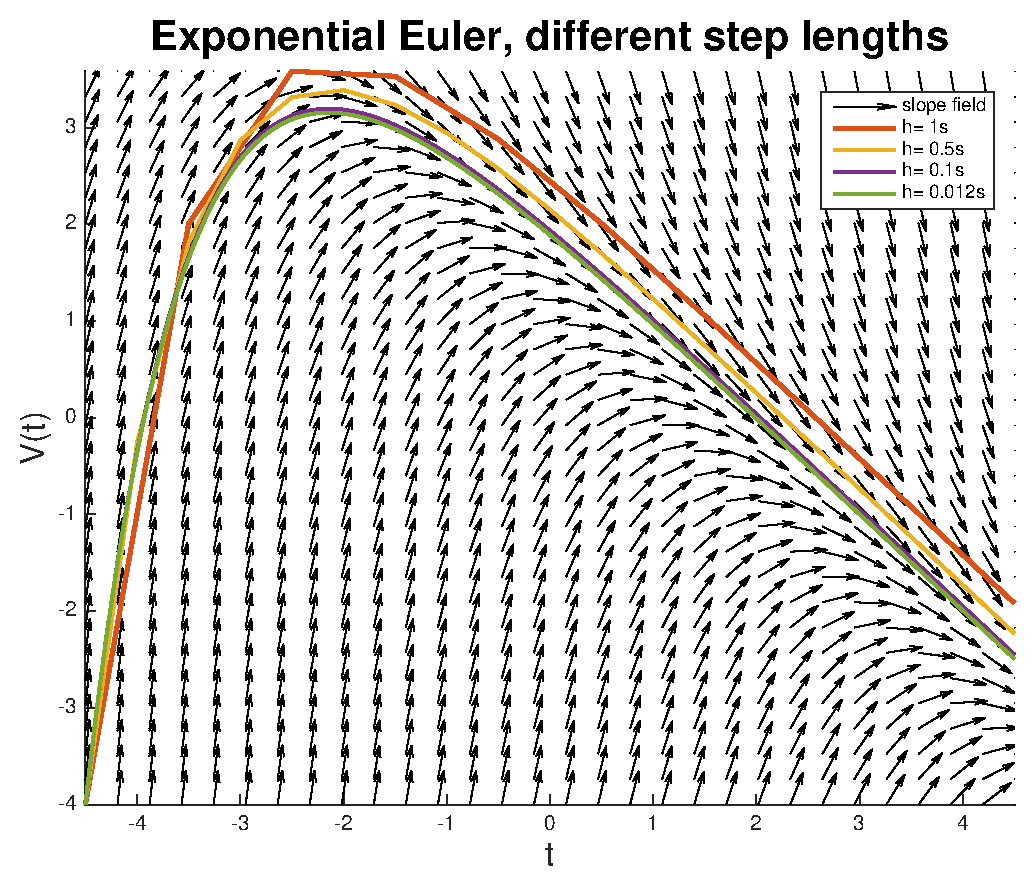
\includegraphics[width=0.85\linewidth]{Plots/ExpEuler}
		\caption{Exponential Euler with different step sizes. The plots for $h = 0.012s$ and $h = 0.1s$ are nearly overlapping and hardly distinguishable. }
		\label{fig:ExpEuler}
	\end{figure}
	
	\subsubsection*{Why not just use a very small step size?}
	The explicit Euler method is a first-order method, which means that the local error (error per step) is proportional to the square of the step size, and the global error is proportional to the step size. Using a small step size thus results in a better approximation and a smaller error. However, a small step size also means a large number of steps in total, which entails a \textit{high computational cost}. Furthermore, for rapidly changing functions, a small step size could even increase the error. Therefore, other approximations, such as the Runge-Kutta methods are needed. 
	
	
	
	\subsection{The Leaky Integrate and Fire Neuron}
	\begin{figure}[h]
\centering
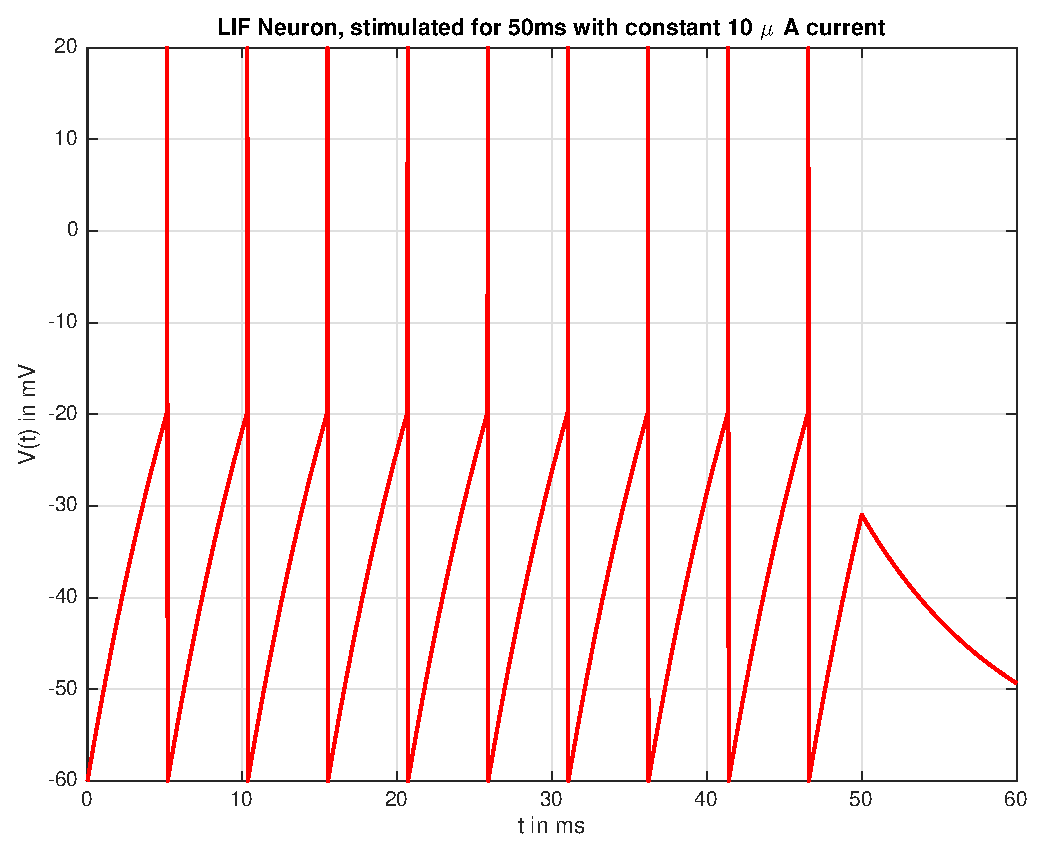
\includegraphics[width=0.7\linewidth]{Plots/LIF_10c}
\caption{LIF neuron stimulated for 50 ms with constant current $I=10\mu$A}
\label{fig:LIF_10c}
\end{figure}

\begin{figure}[h]
	\centering
	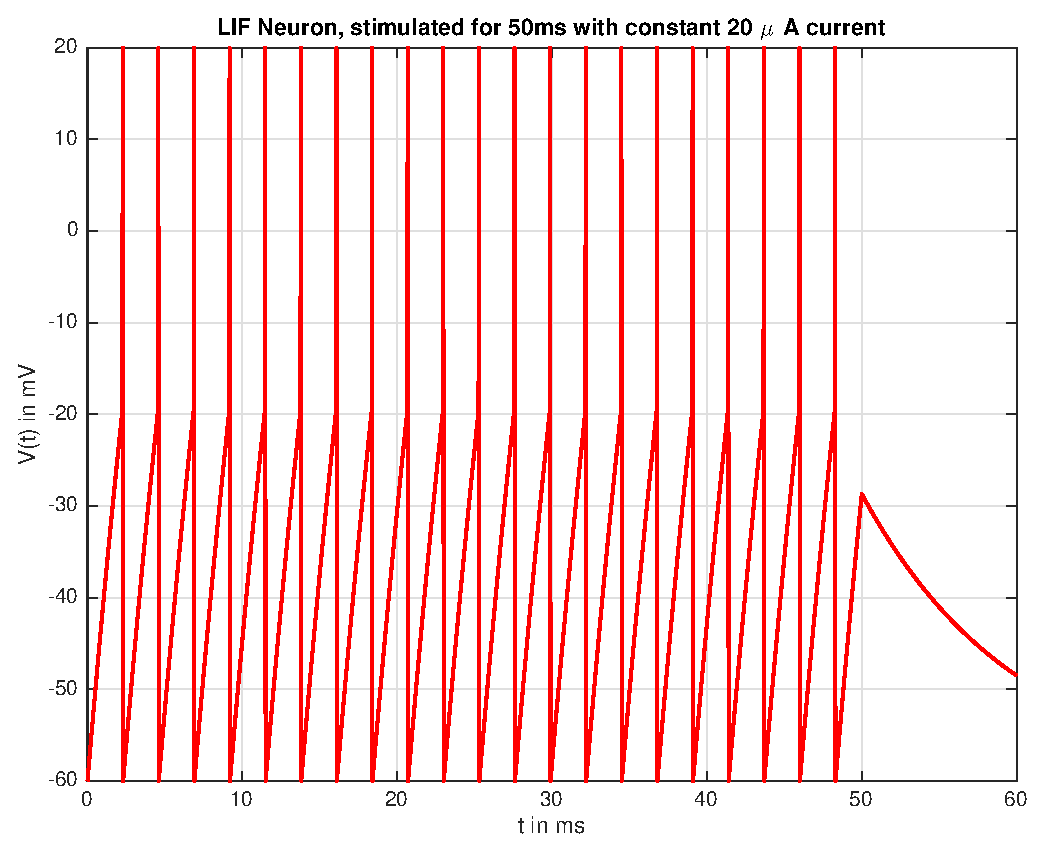
\includegraphics[width=0.7\linewidth]{Plots/LIF_20c}
	\caption{LIF neuron stimulated for 50 ms with constant current $I=20\mu$A}
	\label{fig:LIF_20c}
\end{figure}

\begin{figure}[h]
	\centering
	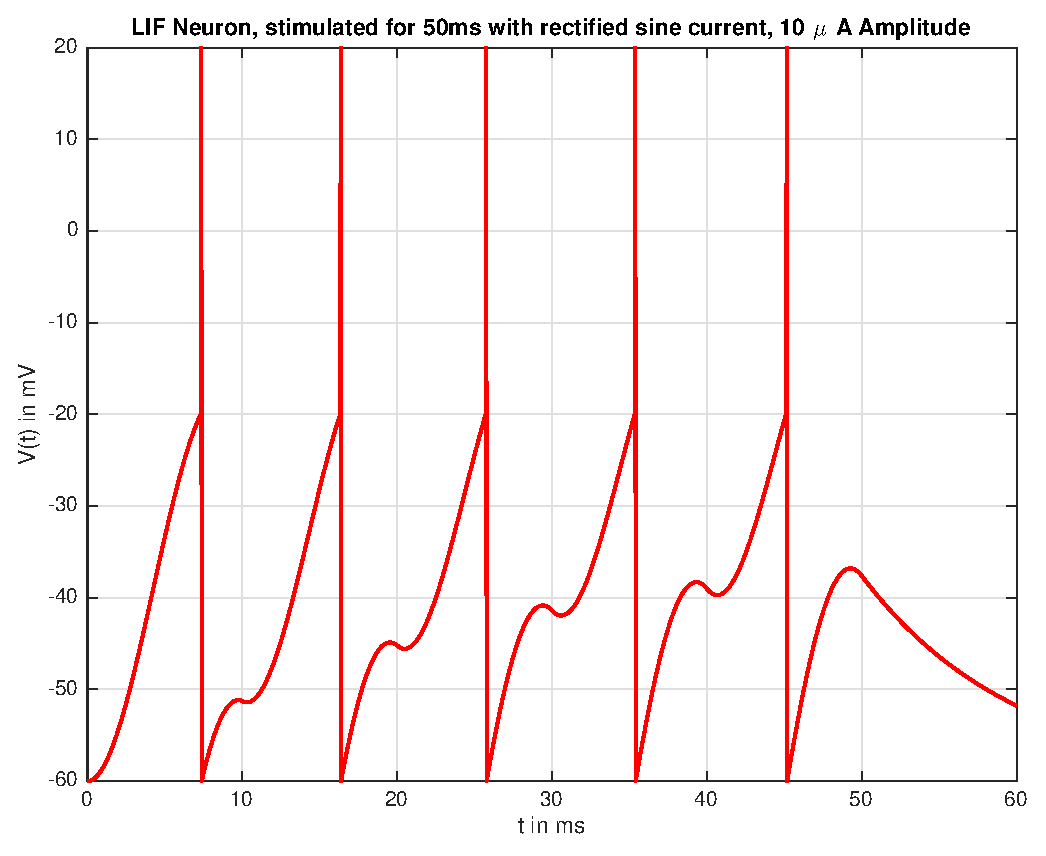
\includegraphics[width=0.7\linewidth]{Plots/LIF_10s}
	\caption{LIF neuron stimulated for 50 ms with rectified sine current, $A = 10\mu$A Amplitude.}
	\label{fig:LIF_10s}
\end{figure}

\begin{figure}[h]
	\centering
	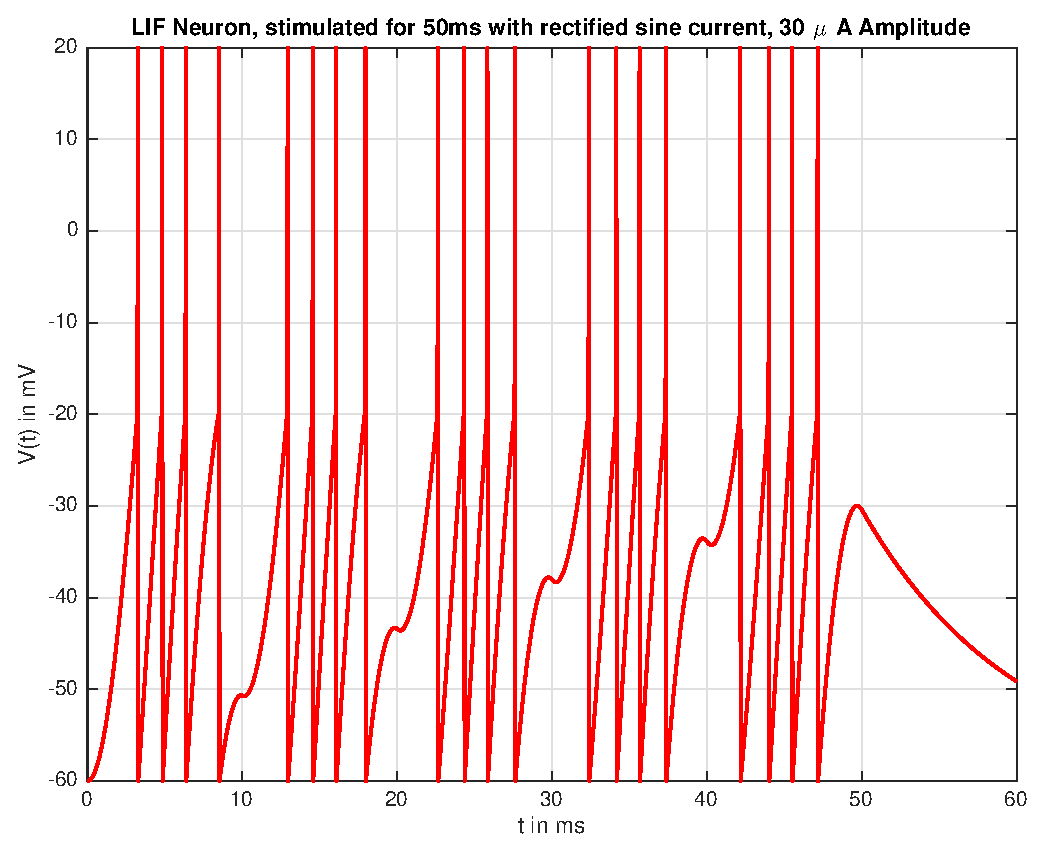
\includegraphics[width=0.7\linewidth]{Plots/LIF_30s}
	\caption{LIF neuron stimulated for 50 ms with rectified sine current, $A = 30\mu$A Amplitude.}
	\label{fig:LIF_30s}
\end{figure}

\subsubsection*{Interpretation of the results}
The \textit{leaky integrate and fire} (LIF) neuron is mere passive description of the membrane. The current that is applied to the neurons may be thought of as a patch electrode inserted into the neuron.\\
The neuron model integrates over the input current by charging the membrane capacitance. When reaching a threshold voltage of $V_m = -20$ mV, the neuron spikes to $V_{spike} = 20$ mV (e.g. see figure 4, where this is nicely visible). After having spiked, the neuron's membrane potential is reset to $V_m = V_{rest} = -60$ mV, and the integration of the persistent input current reoccurs, resulting in a recurrent spiking in fixed intervals (see figure 4 for example). When comparing figures 4 and 5, we notice that the neuron spikes more often when stimulated with a higher current ($10\mu$A vs. $20\mu$A). This model sets no limits in spiking frequency, which is unrealistic. A real neuron has a refractory time of at least 1 to 2 ms, so the maximum spiking frequency response would be between 500 and 1000 Hz.\\
The same holds for figures 6 and 7, where a rectified sine was applied. However, here we see \emph{bumps} in the integration phase. This is due to the input current going very low periodically due to its sine nature, and the \emph{leaky} part (discharging of the membrane capacitance) of the model is stronger than the charging of the membrane capacitance for a very short time. When the sine rises again up to its amplitude value, the membrane capacitance potential reaches the threshold value and the neuron spikes a several times, while the integrated current is still high enough. \\
\textbf{Edit:} The time window of the plots is between $0$ and $60$ ms, whereas the neuron is only stimulated for $50$ ms. That way, one can better see the discharging of the membrane capacitance through the leak conductance. 
	
	

\end{document}